\documentclass{tufte-handout}

%--------Packages--------
\usepackage{makecell}
\usepackage{amsmath}
\usepackage{amssymb}
\usepackage{amsthm}
\usepackage{mathtools}
\usepackage{bbm}
\usepackage{nicefrac}
\usepackage{enumitem}
\usepackage{cleveref}
\usepackage[italic]{derivative}

\bibliographystyle{plain}

%--------Label sections & subsections-------------
\setcounter{secnumdepth}{2}
% \renewcommand{\thesubsection}{\thesection.\Alph{subsection}}

%--------Theorem Environments--------
\newtheorem{thm}{Theorem}
\newtheorem{cor}[thm]{Corollary}
\newtheorem{lem}[thm]{Lemma}
\newtheorem{clm}[thm]{Claim}

\theoremstyle{definition}
\newtheorem{defn}[thm]{Definition}

\theoremstyle{remark}
\newtheorem{rmk}[thm]{Remark}

%--------Margin Tags-------------
\newcommand{\safefootnote}[1]{\footnotemark \margintag{\textsuperscript{\tiny\arabic{footnote}} #1}}
\let\marginnote\relax
\usepackage{marginnote}
\newcommand{\margintag}[1]{
    \checkoddpage
    \ifoddpage
      {\marginnote{\footnotesize #1}}
    \else
      {\reversemarginpar\marginnote{\footnotesize #1}}
    \fi}

%--------Allow page breaks in align-------------
\allowdisplaybreaks

%--------Enumerations-------------
\setenumerate{label=(\arabic*),noitemsep,topsep=0pt,leftmargin=20pt}
% !TeX root = main.tex
% Add the above to each chapter to make compiling the PDF easier in some editors.

\newcommand{\blankpage}{\newpage\hbox{}\thispagestyle{empty}\newpage}
\newcommand{\emptyparagraph}{\paragraph{}\noindent}

\NewDocumentCommand{\floor}{m}{\ensuremath{\left\lfloor #1 \right\rfloor}}
\NewDocumentCommand{\ceil}{m}{\ensuremath{\left\lceil #1 \right\rceil}}

\NewDocumentCommand{\abs}{m}{\ensuremath{\left| #1 \right|}}
\NewDocumentCommand{\norm}{m}{\ensuremath{\left\| #1 \right\|}}
\NewDocumentCommand{\dvm}{m}{\ensuremath{\left( #1 \right)^\#}}

\NewDocumentCommand{\defeq}{}{\overset{.}{=}}
\NewDocumentCommand{\eqdef}{}{\overset{.}{=}}

\DeclareMathOperator*{\im}{im}

\DeclareMathOperator*{\argmax}{arg\,max}
\DeclareMathOperator*{\argmin}{arg\,min}
\DeclareMathOperator*{\as}{\overset{\mathrm{a.s.}}{=}}

\DeclarePairedDelimiter\parentheses{(}{)}
\DeclarePairedDelimiter\brackets{[}{]}
\DeclarePairedDelimiter\braces{\{}{\}}

\newcommand{\R}{\mathbb{R}}
% \newcommand{\Rzero}{\mathbb{R}_{\geq 0}}
\newcommand{\Nat}{\mathbb{N}}

% \newcommand{\MLE}{\mathrm{MLE}}
% \newcommand{\MAP}{\mathrm{MAP}}
% \newcommand{\train}{\mathrm{train}}
% \newcommand{\val}{\mathrm{val}}
% \newcommand{\id}{\mathrm{id}}

\newcommand{\trans}[1]{{#1}^\top}
\newcommand{\compl}[1]{{#1}^\bottom}

\newcommand{\s}[1]{#1^*}

\renewcommand{\vec}[1]{\mathbold{#1}}
\newcommand{\mat}[1]{\mathbold{#1}}
\newcommand{\rvec}[1]{\mathbf{#1}}
\newcommand{\set}[1]{#1}
\newcommand{\spa}[1]{\mathcal{#1}}

\newcommand{\grad}{\nabla\!\!\!\!\!\nabla}
\newcommand{\iti}{{\infty\to\infty}}

% \newcommand{\mean}[1]{\overline{#1}}
% \newcommand{\old}[1]{#1^{\mathrm{old}}}

% common operators
\RenewDocumentCommand{\Pr}{m}{\mathbb{P}\brackets*{#1}}
\NewDocumentCommand{\Ind}{m}{\mathbb{1}\{{#1}\}}
\NewDocumentCommand{\E}{somo}{\ensuremath{\mathbb{E}\IfValueT{#2}{_{#2}}{} \IfBooleanTF{#1}{#3}{\IfValueTF{#4}{\left[#3\ \middle|\ #4\right]}{\brackets*{#3}}}}}
% \NewDocumentCommand{\Var}{som}{\mathrm{Var}\IfValueT{#2}{_{#2}}{} \IfBooleanTF{#1}{#3}{\brackets*{#3}}}
% \NewDocumentCommand{\Cov}{som}{\mathrm{Cov}\IfValueT{#2}{_{#2}}{} \IfBooleanTF{#1}{#3}{\brackets*{#3}}}
\NewDocumentCommand{\KL}{mm}{\mathrm{KL}\parentheses*{#1 \| #2}}
\NewDocumentCommand{\JS}{m}{\mathrm{JS}\parentheses*{#1}}
\NewDocumentCommand{\LandauO}{m}{\mathcal{O}\parentheses*{#1}}
\NewDocumentCommand{\TildeLandauO}{m}{\Tilde{\mathcal{O}}\parentheses*{#1}}
\NewDocumentCommand{\LandauOmega}{m}{\ensuremath{\Omega\parentheses*{#1}}}
\NewDocumentCommand{\LandauTheta}{m}{\ensuremath{\Theta\parentheses*{#1}}}
\NewDocumentCommand{\gap}{}{\mathrm{gap}}
% \NewDocumentCommand{\determ}{m}{|#1|}
% \NewDocumentCommand{\tr}{m}{\mathrm{tr}\parentheses*{#1}}
\NewDocumentCommand{\diag}{}{\mathrm{diag}}
% \NewDocumentCommand{\pset}{m}{\mathcal{P}\parentheses*{#1}}

% common vectors, matrices, random vectors, spaces
\newcommand{\vZero}{\vec{0}}
\newcommand{\vOne}{\vec{1}}
\newcommand{\vb}{\vec{b}}
\newcommand{\vc}{\vec{c}}
\newcommand{\vd}{\vec{d}}
\newcommand{\vdelta}{\vec{\delta}}
\newcommand{\ve}{\vec{e}}
\newcommand{\vepsilon}{\vec{\epsilon}}
\newcommand{\vf}{\vec{f}}
\newcommand{\vg}{\vec{g}}
\newcommand{\vmu}{\vec{\mu}}
\newcommand{\vphi}{\vec{\phi}}
\newcommand{\vpsi}{\vec{\psi}}
\newcommand{\vtheta}{\vec{\theta}}
\newcommand{\vv}{\vec{v}}
\newcommand{\vx}{\vec{x}}
\newcommand{\vy}{\vec{y}}
\newcommand{\vz}{\vec{z}}
\newcommand{\rX}{\rvec{X}}
\newcommand{\rY}{\rvec{Y}}
\newcommand{\rZ}{\rvec{Z}}
\newcommand{\mA}{\mat{A}}
\newcommand{\mB}{\mat{B}}
\newcommand{\mH}{\mat{H}}
\newcommand{\mI}{\mat{I}}
\newcommand{\mJ}{\mat{J}}
\newcommand{\mL}{\mat{L}}
\newcommand{\mM}{\mat{M}}
\newcommand{\mP}{\mat{P}}
\newcommand{\mSigma}{\mat{\Sigma}}
\newcommand{\mU}{\mat{U}}
\newcommand{\sA}{\set{A}}
\newcommand{\sB}{\set{B}}
\newcommand{\sX}{\set{X}}

\newcommand{\lmin}{\lambda_{\mathrm{min}}}
\newcommand{\lmax}{\lambda_{\mathrm{max}}}

% distributions
\NewDocumentCommand{\N}{omm}{\mathcal{N}(\IfValueT{#1}{#1;}{} #2, #3)}
\NewDocumentCommand{\SN}{o}{\mathcal{N}(\IfValueT{#1}{#1;}{} \vzero, \mI)}
\NewDocumentCommand{\uSN}{o}{\mathcal{N}(\IfValueT{#1}{#1;}{} 0, 1)}
\NewDocumentCommand{\GP}{omm}{\mathcal{GP}(\IfValueT{#1}{#1;}{} #2, #3)}
\NewDocumentCommand{\Unif}{om}{\mathrm{Unif}(\IfValueT{#1}{#1;}{} #2)}
\NewDocumentCommand{\Bern}{om}{\mathrm{Bern}(\IfValueT{#1}{#1;}{} #2)}
\NewDocumentCommand{\Bin}{omm}{\mathrm{Bin}(\IfValueT{#1}{#1;}{} #2, #3)}
\NewDocumentCommand{\Beta}{omm}{\mathrm{Beta}(\IfValueT{#1}{#1;}{} #2, #3)}


\title{Probabilistic Generative Models}
\author{Jonas Hübotter}
\date{May 7th, 2022}

\begin{document}
\maketitle

This is intended as an introduction to the use of uncertainty in generative models. We will start without assuming any prior knowledge of generative models and progress quickly to discuss the most fundamental ideas behind some of the most powerful generative models to date.

\section{Generative Models}

A generative model is a model that learns to imitate some pattern-generating process. That is, we have (high-dimensional) patterns $\vx \in \spa{X}$ that are generated according to a probability distribution $p$ on $\spa{X}$. We want to learn a model $p_\vtheta$ that is indistinguishable from $p$. In particular, our model should \begin{enumerate}
    \item avoid missing patterns that are generated by $p$ (this is called \emph{mode collapse}) and
    \item avoid generating patterns that are not supported by $p$.
\end{enumerate}

A famous example is the example of generating human faces, where we want to generate facial features proportional to how frequently they occur in real human faces.

\subsection{Density Estimation}

The problem as stated is above is also called a \emph{density estimation} problem, that is, we want to estimate a density $p$ using a family of densities $p_\vtheta$ parametrized by $\vtheta$. The canonical method for parameter estimation (also called inference) is \emph{maximum likelihood estimation}, for short. In MLE, we pick $\vtheta$ such that it explains the patterns generated by $p$ best, \begin{align}
    \s{\vtheta} &= \argmax_\vtheta \E[\vx \sim p]{p_\vtheta(\vx)} \\
    &= \argmax_\vtheta \E[\vx \sim p]{\log p_\vtheta(\vx)}. \margintag{using monotonicity of the logarithm}
\end{align} $p_\vtheta(\vx)$ is also called the \emph{evidence} of $\vx$. So maximum likelihood estimation corresponds to maximizing the evidence of $\vx$ under the model $p_\vtheta$ when $\vx$ is sampled according to the true distribution $p$.

Given that we can differentiate $p_\vtheta(\vx)$ with respect to $\vtheta$, we can easily obtain unbiased gradient estimates, which we can use to find a sample-based approximation of $\s{\vtheta}$.\footnote{Because we can only use finitely many samples $\vx$, picking a single point estimate of $\hat{\vtheta}$ might not be the best choice. Often, it is helpful to encode the uncertainty in our choice of $\s{\vtheta}$ using a distribution.}

Learning a density $p$ directly --- for example using standard techniques from deep learning --- is hard. This is because our model has to fulfill structural constraints to be a valid density. Moreover, learning the densities directly does not allow us to efficiently sample from the resulting distribution.

Simple parametric models such as \emph{autoregressive models}, which break down the problem of generating $\vx$ into the problem of sequentially generating components $\vx(i)$ given previously generated components $\vx(1),\dots,\vx(i-1)$, turn out not to be expressive enough for challenging, high-dimensional generative tasks.\footnote{Autoregressive models are very useful for time-series prediction.} We have seen that throwing deep neural networks (DNNs) at the task directly is not very useful, but we do need their expressiveness for modeling $p$ accurately.

\subsection{Implicit Models}

A useful approach to make DNNs work in a constrained setting, is to encode the constraints implicitly in our model. This idea leads to the family of \emph{implicit models}, where we generate $\vx$ by first generating a random vector $\vz$ from a known distribution $\spa{D}$ and then use a deterministic DNN $\vf_\vtheta$ with parameters $\vtheta$ to ``lift'' $\vz$ into the set of patterns $\spa{X}$. We can think of this as a transformation of random vectors, \begin{align}
    \rX \defeq \vf_\vtheta(\rZ), \quad \rZ \sim \spa{D}.
\end{align} Often, we sample the \emph{encoding} $\vz$ according to the standard normal distribution, $\spa{D} \defeq \N{\vZero}{\mI}$.

\begin{marginfigure}
    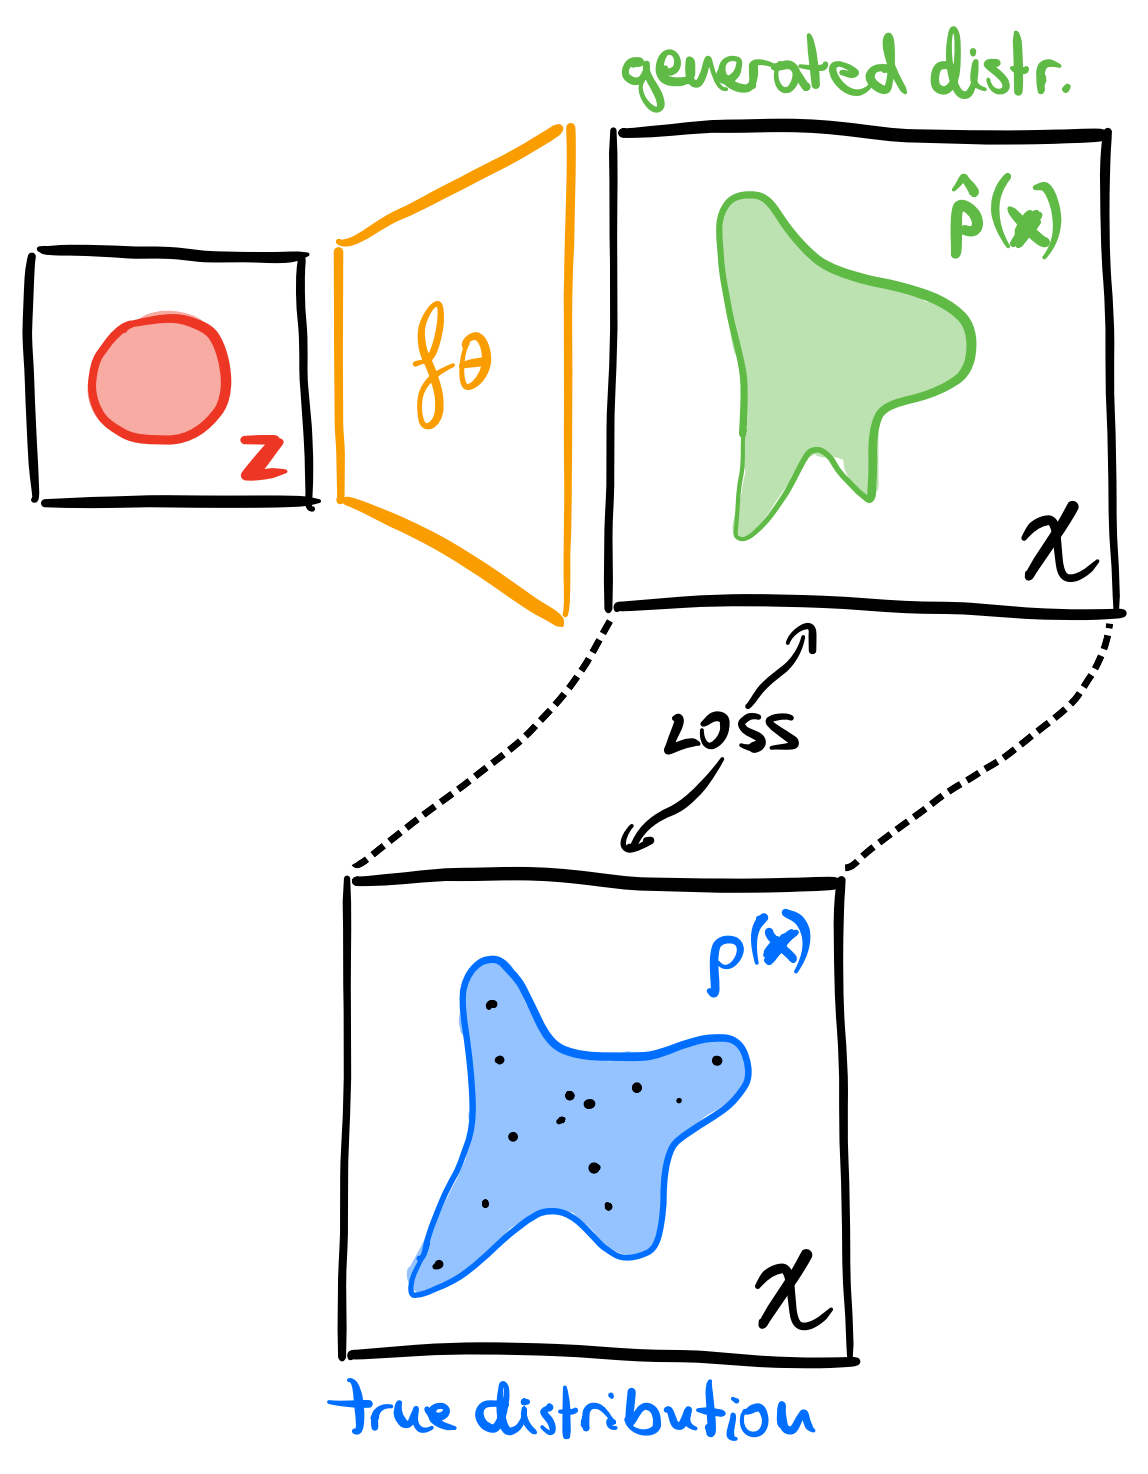
\includegraphics[width=\textwidth]{figures/implicit_model.png}
    \caption{An implicit model ''lifts`` $\vz$ from the \emph{code space} (also called \emph{latent space}) to the \emph{pattern space} using a DNN $\vf$ parametrized by $\vtheta$.}
\end{marginfigure}

For general DNNs $\vf$, parameter estimation becomes intractable. To perform parameter estimation, we need to recover the density $p_\vtheta$ of our model. This can be done using so-called \emph{pushforward measures} when $\vf$ is invertible and it is easy to compute $\det \mJ_\vf$, where $\mJ_\vf$ is the Jacobian of $\vf$. Such $\vf$ are also called \emph{normalizing flows}.\footnote{We will not go into more depth on normalizing flows here.}

\subsection{Outline}

Normalizing flows restrict the architecture of the DNN $\vf$ to ensure that recovering the density, and thus inference, remains tractable. An alternative approach is to perform inference approximately. This approach, we will discuss in the next section on \emph{variational autoencoders}.

Finally, we will look at a different and very powerful class of models known as \emph{generative adversarial models}.

\section{Variational Autoencoders}

One common approach to perform approximate inference is to maximize a lower bound on the evidence instead of maximizing this evidence directly. To obtain a lower bound on the log-evidence $\log p_\vtheta(\vx)$, we can relate this quantity back to the space of encodings: \begin{align}
    \log p_\vtheta(\vx) &= \log \int p_\vtheta(\vx \mid \vz) p(\vz) \,d\vz. \nonumber
\intertext{Intuitively, the probability of $\vx$ is the probability of an encoding $\vz$ being ``lifted'' to $\vx$ times the probability of the encoding $\vz$ to be sampled in the first place.\safefootnote{The true distribution over the latent space $p(\vz)$ is not to be confused with the true distribution over the pattern space $p(\vx)$.} We can rewrite this to,}
    &= \log \int p_\vtheta(\vx \mid \vz) \frac{p(\vz)}{q(\vz)} q(\vz) \,d\vz \nonumber \\
    &= \log \E[\vz \sim q]{p_\vtheta(\vx \mid \vz) \frac{p(\vz)}{q(\vz)}}, \nonumber
\intertext{where $q$ is any density on the code space. Using Jensen's inequality and that $\log$ is concave, we obtain,}
    &\geq \E[\vz \sim q]{\log p_\vtheta(\vx \mid \vz)} - \E[\vz \sim q]{\log \frac{q(\vz)}{p(\vz)}}.
\end{align} This lower bound on the log-evidence is also known as the \emph{evidence lower bound} (or ELBO for short).

\begin{marginfigure}[-10\baselineskip]
    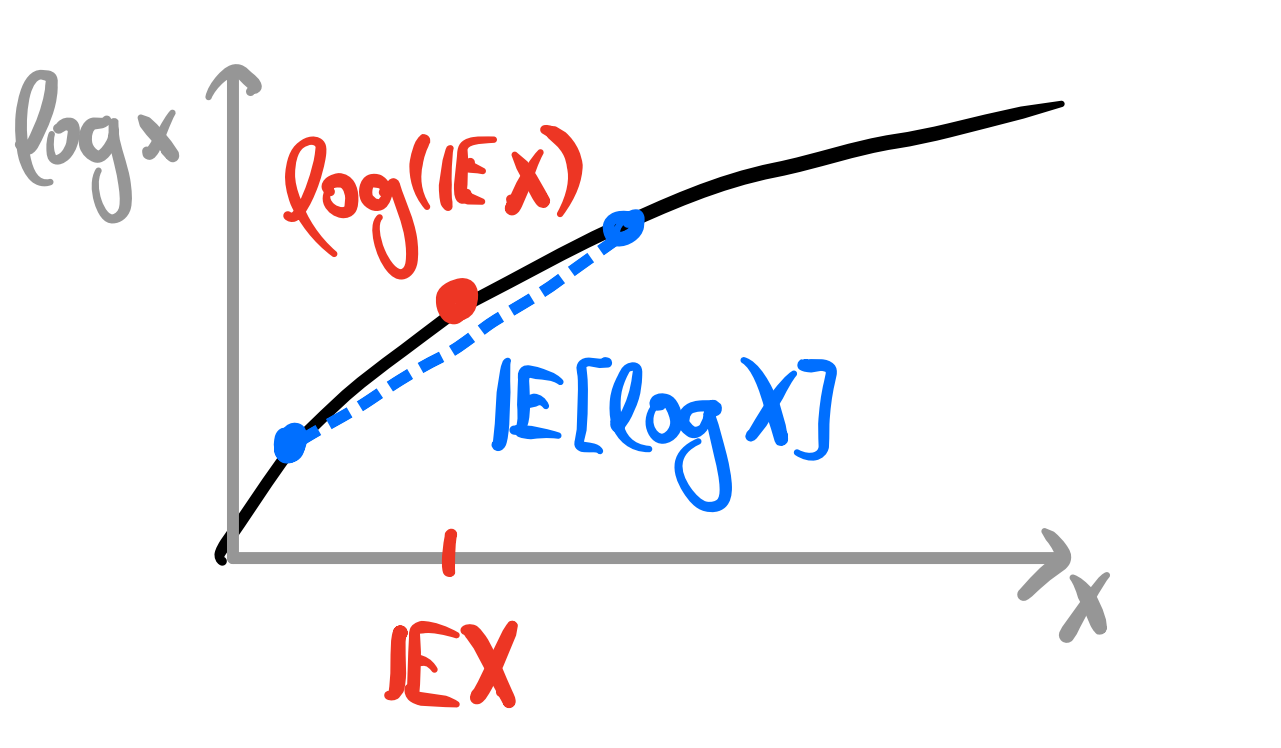
\includegraphics[width=\textwidth]{figures/jensen.png}
    \caption{An illustration of Jensen's inequality.}
\end{marginfigure}

The regularization term $\E[\vz \sim q]{\log \frac{q(\vz)}{p(\vz)}}$ is also called \emph{(reverse) Kullback-Leibler divergence}, $\KL{q}{p}$, and measures how well $q$ approximates the true distribution of encodings $p$. Maximizing ELBO therefore corresponds to maximizing the likelihood of $\vx$ given samples of encodings $\vz$, while $\vz$ are sampled according to a distribution $q$, which is close to $p$. When $q$ is from a class of distributions parametrized by $\vpsi$, then $q_\vpsi$ is also called a \emph{variational distribution}.

\begin{figure}
    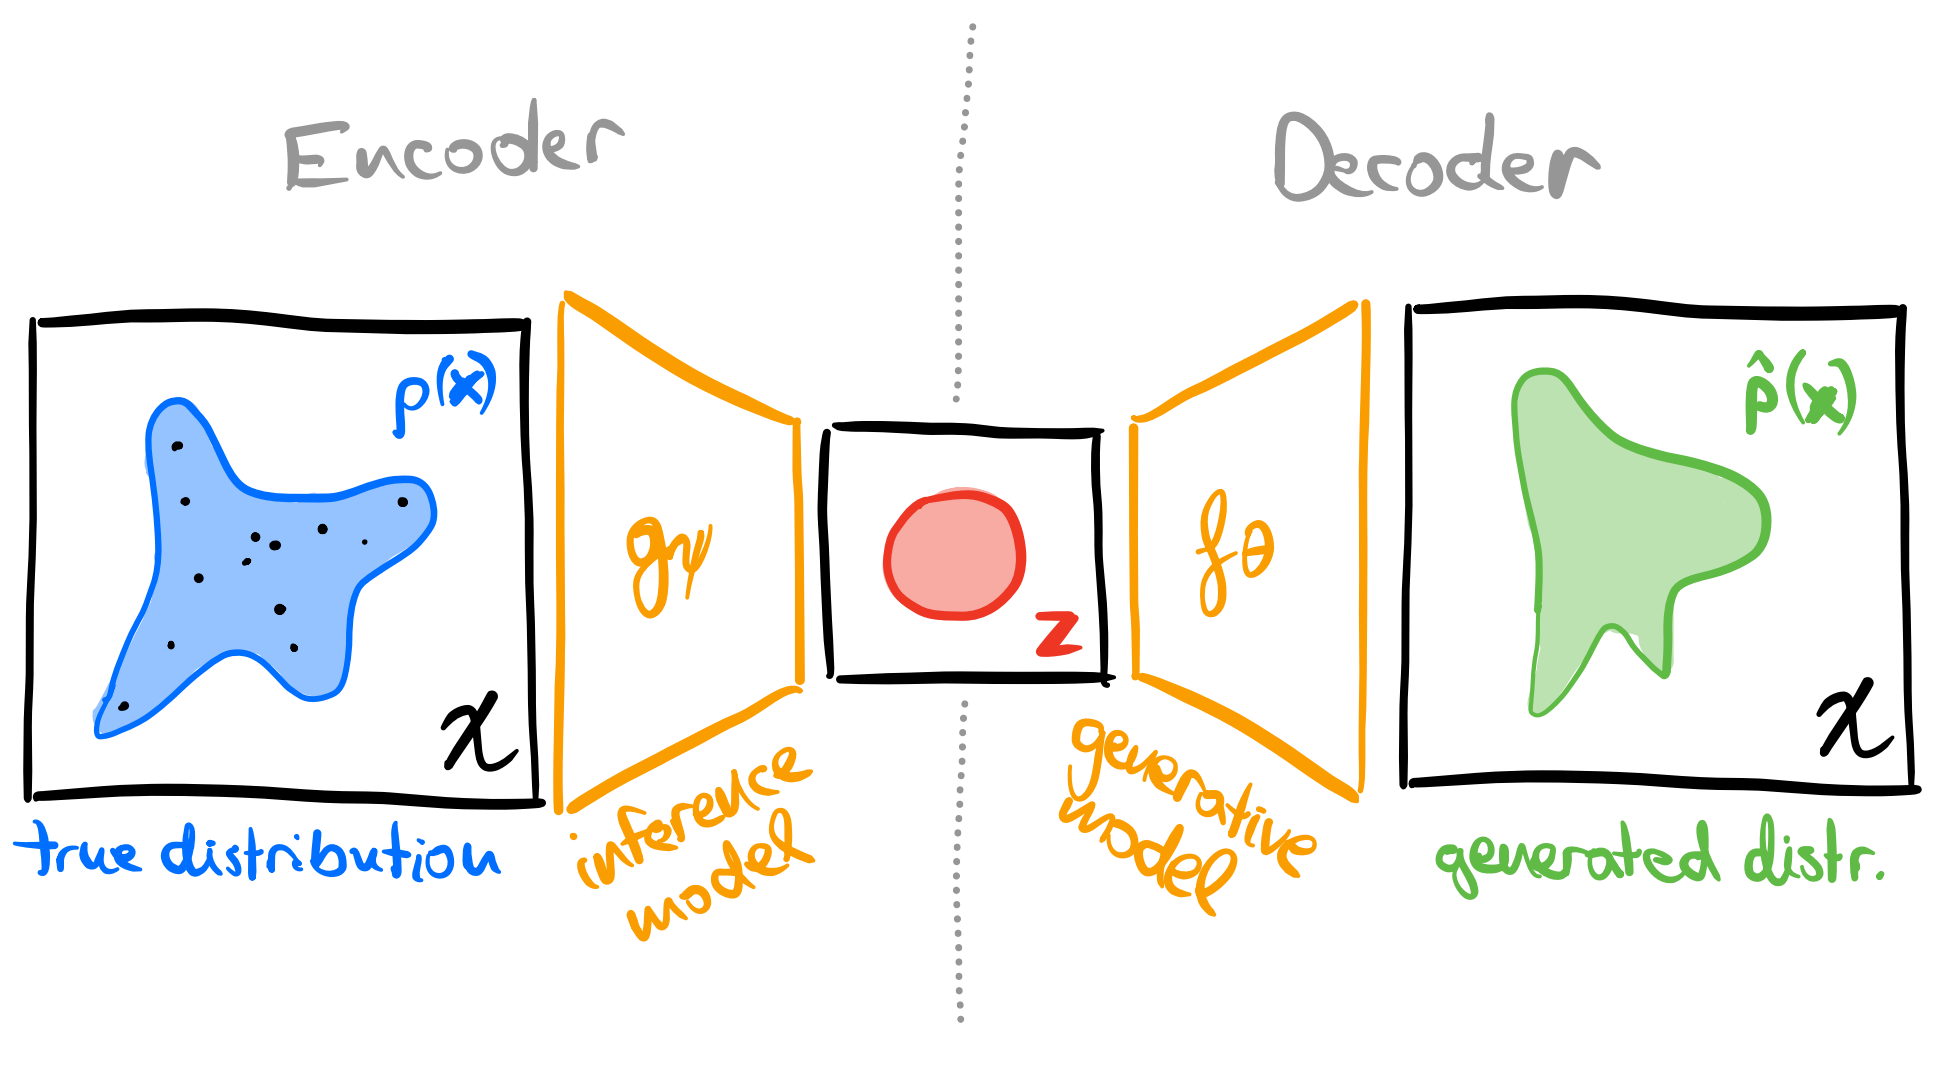
\includegraphics[width=\textwidth]{figures/vae.png}
    \caption{A variational autoencoder learns an inference model and generative model simultaneously. The learned inference model is used to produce encodings from which the generative model should produce patterns.}
\end{figure}

The key idea of variational autoencoders is to simultaneously learn a generative model $p_\vtheta$ and inference model $q_\vpsi$. So given a pattern $\vx$ sampled according to the true distribution of patterns $p$, the objective to be maximized is, \begin{align}
    \log p_\vtheta(\vx) \gtrapprox  \E[\vz \sim q_\vpsi(\cdot \mid \vx)]{\log p_\vtheta(\vx \mid \vz)} - \KL{q_\vpsi(\cdot \mid \vx)}{p} \eqdef \ell(\vtheta, \vpsi; \vx).
\end{align} The KL-divergence can often be expressed analytically, and we can use a sample-based approximation for the expectation.

\subsection{The Inference Model}

You may (rightfully) object that we have simply extended our task of finding a generative model $p_\vtheta$ by finding yet another generative model $\vg_\vpsi$. However, the latter generative model is from a high- to a low-dimensional space, namely from the pattern space to the code space. It turns out that this task is much simpler than the task that we started with.

Typically, the inference model is chosen to be a non-isotropic statistical transformation of the outputs of a DNN. More concretely, we use a DNN $\vg_\vpsi$ to first transform the high-dimensional pattern $\vx$ to a low-dimensional feature representation and then to outputs $\vmu_\vpsi$ and $\mSigma_\vpsi$.\footnote[][-1\baselineskip]{For example, by using a convolutional neural network to obtain the feature representation and a fully connected neural network to learn mappings to $\vmu_\vpsi$ and $\mSigma_\vpsi$.} We then choose $q_\vpsi$ to be a simple distribution with mean $\vmu_\vpsi$ and covariance $\mSigma_\vpsi$ (i.e., $\N{\vmu_\vpsi}{\mSigma_\vpsi}$) that is easy to sample from.

\begin{figure}
    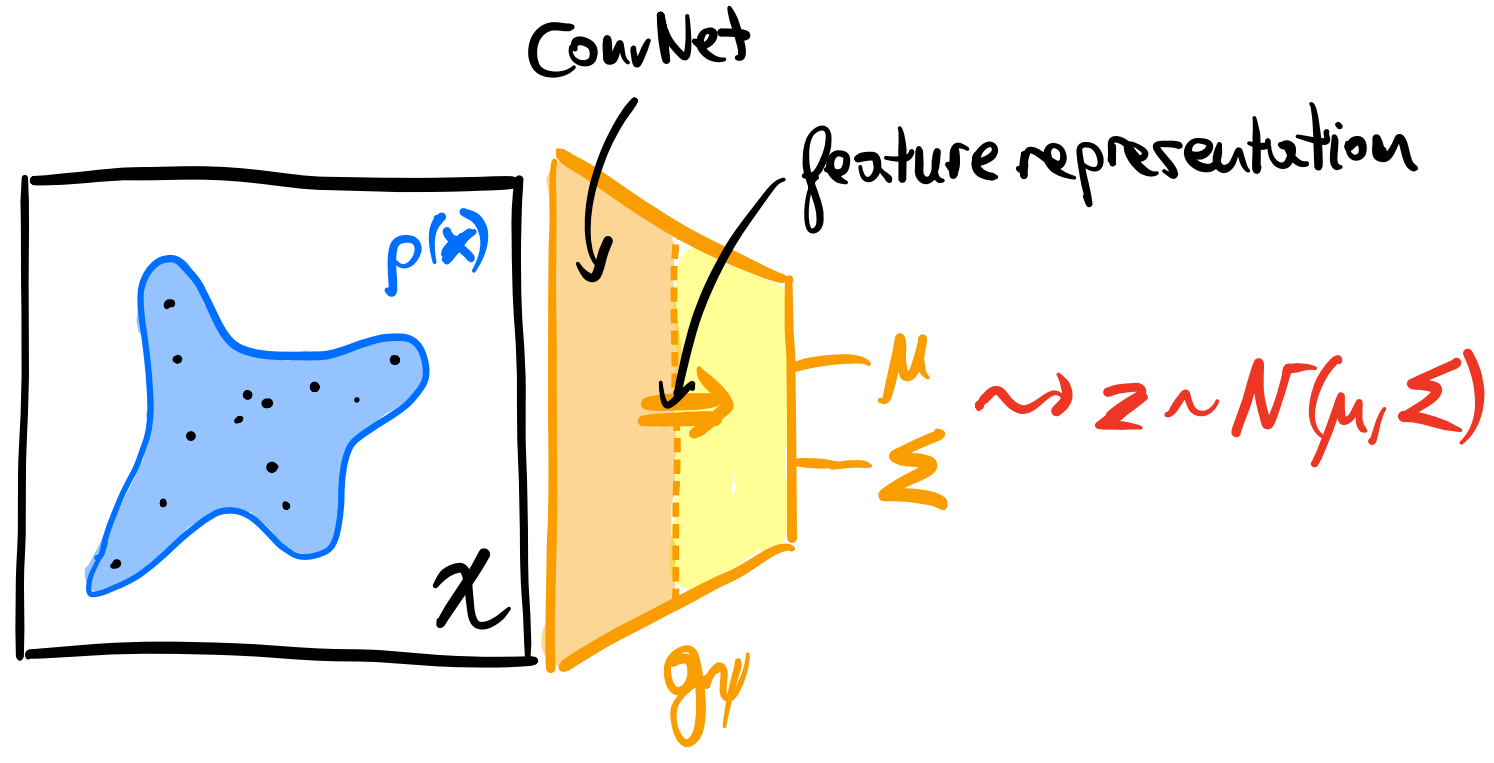
\includegraphics[width=\textwidth]{figures/inference_model.png}
    \caption{Illustration of a typical inference model. First, a pattern is transformed into a feature representation, which is then used to obtain statistics $\vmu$ and $\mSigma$ that parametrize a distribution over encodings.}
\end{figure}

We call such a model \emph{non-isotropic} because the statistics $\vmu_\vpsi$ and $\mSigma_\vpsi$ depend on the pattern $\vx$.

\subsection{Inference}

Now, to perform inference, we need to be able to obtain gradients with respect to $\vtheta$ and $\vpsi$ of $\ell(\vtheta, \vpsi; \vx)$. As we mentioned, the KL-divergence can usually be expressed analytically. This is also true for its gradient. The gradient of $p_\vtheta(\vx \mid \vz)$ can be computed using backpropagation. The difficulty lies in finding the gradient of the expectation $\E[\vz \sim q_\vpsi(\cdot \mid \vx)]{\log p_\vtheta(\vx \mid \vz)}$ with respect to $\vpsi$. Because the expectation integrates over a measure that depends on the parameters $\vpsi$, we cannot simply draw the gradient into the expectation using linearity.

Here, we can use the so-called \emph{reparameterization trick} by writing $\vz \sim q_\vpsi(\cdot, \vx) = \N{\vmu_\vpsi}{\mSigma_\vpsi}$ as, \begin{align}
    \vz = \vmu_\vpsi + \mSigma_\vpsi^{\nicefrac{1}{2}}\vepsilon, \quad \vepsilon \sim \N{\vZero}{\mI},
\end{align} where $\vmu_\vpsi$ and $\mSigma_\vpsi$ are the outputs of the DNN $\vg_\vpsi$. We obtain, \begin{align}
    \E[\vz \sim q_\vpsi(\cdot \mid \vx)]{\log p_\vtheta(\vx \mid \vz)} = \E[\vepsilon \sim \N{\vZero}{\mI}]{\log p_\vtheta(\vx \mid \vmu_\vpsi + \mSigma_\vpsi^{\nicefrac{1}{2}}\vepsilon)}.
\end{align} Of this expectation, we can now easily obtain unbiased gradient estimates, which we can use to maximize the ELBO using stochastic gradient descent. For more details on the reparameterization trick for Gaussians or other distributions and the computation of gradients of the ELBO, refer to section 5.2.7 of my notes on probabilistic artificial intelligence.

\begin{figure}
    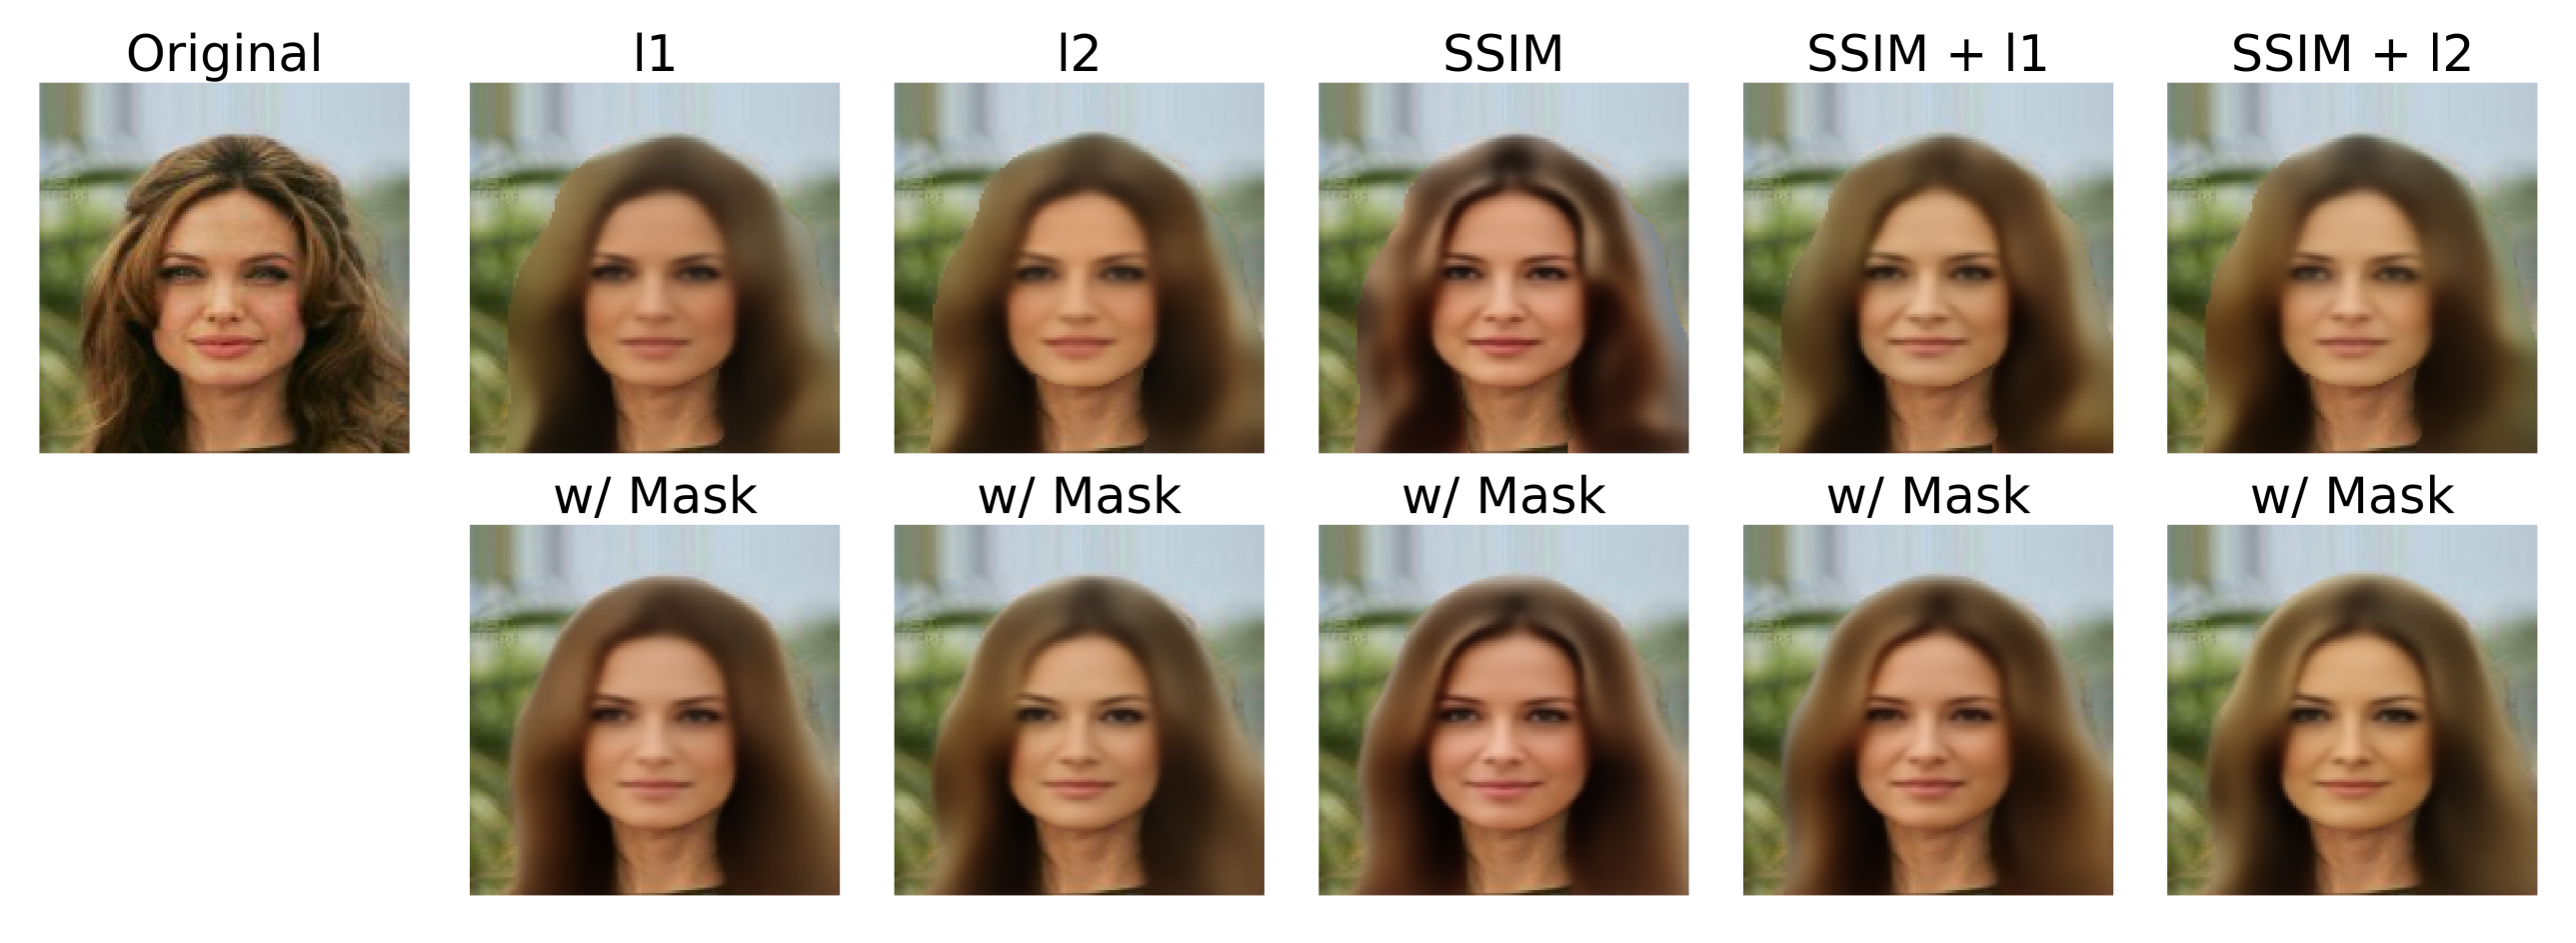
\includegraphics[width=\textwidth]{figures/faces_vae.png}
    \caption{An example of faces reconstructed by a variational autoencoder. Taken from \citep{toledo2021face}.}
\end{figure}

\section{Generative Adversarial Models}

We will now introduce a different class of models that are based on a very simple and beautiful idea, and which are powerful enough to yield models that produce faces that are visually indistinguishable from real faces.

Recall that our original goal was to find a distribution $p_\vtheta$ that is indistinguishable from the distribution $p$. Our initial instinct was to use density estimation to find $p_\vtheta$, but we have seen that we either have to limit the expressiveness of our model to retain tractability of the inference problem or we have to perform inference approximately. It is therefore useful to think whether we can characterize our problem in a different way.

The notion of indistinguishability leads to a very natural characterization: our goal is to make it virtually impossible for an agent to distinguish between the patterns produced by $p$ and the patterns produced by $p_\vtheta$. From the perspective of such an agent, this is a simple binary classification problem. Our original task can be interpreted as maximizing the loss of this agent, as a large loss corresponds to the scenario where the patterns produced by $p_\vtheta$ cannot be distinguished from the patterns produced by $p$.

We write $Y \defeq \Ind{\text{pattern is ``natural''}}$. Assuming that the classification problem is balanced,\footnote{That is, we present the agent with labels such that $\Pr{Y=1} = \Pr{Y=0} = \nicefrac{1}{2}$.} it can be characterized using the joint density, \begin{align}
    p(\vx, y; \vtheta) = \underbrace{\Pr{Y = y}}_{=\frac{1}{2}}\begin{cases}
        p(\vx) & y = 1 \\
        p_\vtheta(\vx) & y = 0.
    \end{cases}
\end{align}

A classifier $\pi: \R^n \to [0,1], \pi(\vx) \approx \Pr{Y = 1 \mid \vx}$ is also called a \emph{discriminator}. Intuitively, the discriminator provides an error signal to the generative model, hinting at promising regions in the pattern space.

The canonical approach is to model the loss of a discriminator $\pi$ using \emph{binary cross-entropy} (also called a \emph{logistic loss}), \begin{align}
    \ell(\vtheta, \pi) &\defeq \E[\vx, y \sim p(\cdot; \vtheta)]{y \log \pi(\vx) + (1-y) \log (1 - \pi(\vx)} \\
    &= \frac{1}{2} \int p(\vx) \log \pi(\vx) \,d\vx + \frac{1}{2} \int p_\vtheta(\vx) \log(1 - \pi(\vx)) \,d\vx.
\end{align} Our optimization problem is then given as, \begin{align}
    \min_\vtheta \max_\pi \ell(\vtheta, \pi).
\end{align} In words, we want to make the classification task as difficult as possible for the best-possible classifier $\pi$ by tuning $\vtheta$.

The optimal discriminator is a Bayes-optimal classifier $\s{\pi}$, \begin{align}
    \s{\pi}(\vx) = \Pr{Y = 1 \mid \vx} = \frac{p(\vx)}{p(\vx) + p_\vtheta(\vx)}.
\end{align} In practice, we do not have access to this discriminator, as it depends on the true distribution $p$. Nevertheless, we can compute the expected loss of this classifier to confirm our intuition that when this quantity is large, $p_\vtheta$ must be ``almost indistinguishable'' from $p$.  For the Bayes-optimal discriminator $\s{\pi}$, we obtain, \begin{align}
    \ell(\vtheta, \s{\pi}) &= \E[\vx, y \sim p(\cdot; \vtheta)]{y \log \s{\pi}(\vx) + (1-y) \log (1 - \s{\pi}(\vx)} \nonumber\\
    &= \begin{multlined}[t]
        \frac{1}{2} \int p(\vx) [\log p(\vx) - \log(p(\vx) + p_\vtheta(\vx))] \,d\vx \\ + \frac{1}{2} \int p_\vtheta(\vx) [\log p_\vtheta(\vx) - \log(p(\vx) + p_\vtheta(\vx))] \,d\vx
    \end{multlined} \nonumber\\
    &= \begin{multlined}[t]
        \frac{1}{2} \int p(\vx) \log p(\vx) \,d\vx + \frac{1}{2} \int p_\vtheta(\vx) \log p_\vtheta(\vx) \,d\vx \\ - \int \frac{p(\vx) + p_\vtheta(\vx)}{2} \log\parentheses*{\frac{p(\vx) + p_\vtheta(\vx)}{2}} \,d\vx - \log 2
    \end{multlined} \nonumber\\
    &= \begin{multlined}[t]
        \frac{1}{2} \E[\vx \sim p]{\log p(\vx)} + \frac{1}{2} \E[\vx \sim p_\vtheta]{\log p_\vtheta(\vx)} \\ - \E[\vx \sim \frac{1}{2}p + \frac{1}{2}p_\vtheta]{\log\parentheses*{\frac{1}{2}p(\vx) + \frac{1}{2}p_\vtheta(\vx)}} - \log 2
    \end{multlined} \nonumber\\
    &= - \frac{1}{2} H(p) - \frac{1}{2} H(p_\vtheta) + H\parentheses*{\frac{1}{2}p + \frac{1}{2}p_\vtheta} - \log 2,
\end{align} where $H(p) \defeq \E[\vx \sim p]{- \log p(\vx)}$ is the entropy of distribution $p$ and $\frac{1}{2}p + \frac{1}{2}p_\vtheta$ is a convex combination of the distributions $p$ and $p_\vtheta$. The sum of entropies is also known as the \emph{Jensen-Shannon divergence}, \begin{align}
    \JS{p, q} &= \frac{1}{2} \KL{p}{\frac{1}{2}p + \frac{1}{2}q} + \frac{1}{2} \KL{q}{\frac{1}{2}p + \frac{1}{2}q} \\
    &= - \frac{1}{2} H(p) - \frac{1}{2} H(q) + H\parentheses*{\frac{1}{2}p + \frac{1}{2}q}.
\end{align} Consider the case where $p$ and $q$ are the same distribution, then the JS-divergence is zero. The described optimization problem minimizes the JS-divergence, and hence, the ``distance'' between $p$ and $p_\vtheta$.

As mentioned, we cannot compute $\s{\pi}$ directly, nor can we compute the Jensen-Shannon divergence. Nevertheless, the above derivation motivates that replacing $\argmax_\pi \ell(\vtheta, \pi)$ by a learned discriminator that is close to the true optimum $\s{\pi}$ yields a loss that can be used to estimate a good generator. Let us consider a class of discriminators $\pi_\vphi$ that is parametrized by $\vphi$. Assuming this class is expressive enough to cover $\s{\pi}$, we have, \begin{align}
    \ell(\vtheta, \s{\pi}) = \max_\vphi \ell(\vtheta, \vphi),
\end{align} yielding the saddle point problem, \begin{align}
    \s{\vtheta} = \argmin_\vtheta \max_\vphi \ell(\vtheta, \vphi), \quad \s{\vphi} = \argmax_\vphi \ell(\s{\vtheta}, \vphi).
\end{align} Under conditions of Nash's existence theorem for Nash equilibria, the above is equivalent to, \begin{align}
    \s{\vtheta} = \argmin_\vtheta \ell(\vtheta, \s{\vphi}), \quad \s{\vphi} = \argmax_\vphi \ell(\s{\vtheta}, \vphi).
\end{align} This formulation of generative models is known as \emph{Generative Adversarial Networks} (GANs). We can think of this problem as a two player game with the generator trying to choose $\vtheta$ so as to minimize the loss and the adversary (i.e., the discriminator) trying to choose $\vphi$ so as to maximize the loss.

\begin{figure}
    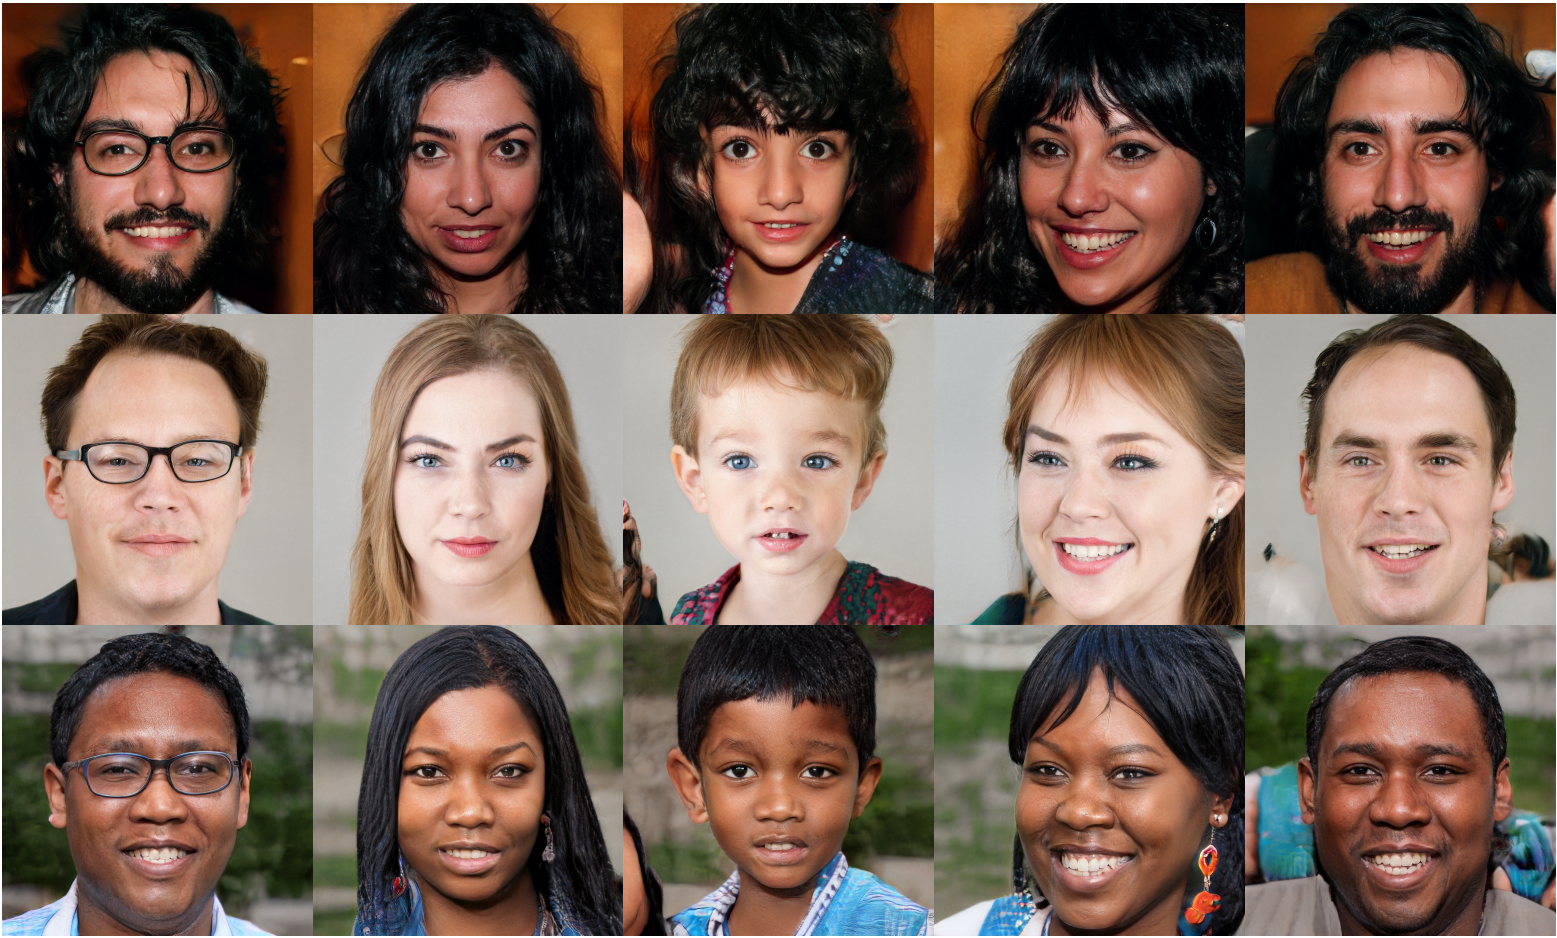
\includegraphics[width=\textwidth]{figures/faces_gans.png}
    \caption{An example of faces constructed by a generative adversarial model, StyleGAN. Taken from \citep{karras2019style}.}
\end{figure}

\nocite{*}
\bibliography{sources}
\end{document}
